\section{Account-level capital}\label{sec:account}

Lemma~\ref{thm:capital} gives the order but not the constant. This section computes what a trader actually needs under a calibrated linear-impact environment, then converts it to Bitcoin dollars.

\paragraph{Numerical status.} The analytic inequalities below are conditional mathematical bounds. The displayed decimal optima and brackets are numerical evaluations, not independently outward-certified enclosures of the continuous frequency or angle extrema. A finite grid and a matching archived number do not establish that enclosure; rigorous optimization remains a separate verification obligation.

\subsection{Observation design and the tri-region partition}

An observer distinguishes two candidate mechanisms with rates $\theta_0$ and $\theta_1=\theta_0+\delta$ over $N$ periods, submitting probes $V=(V_1,\ldots,V_N)^\top$ that generate inventory $I_t=\sum_{s\le t}V_s$. Under contract $I_0$ (active probing, Gaussian observation noise) $p_t=(h_i*V)_t+\epsilon_t$, $\epsilon_t\sim N(0,\sigma^2)$, so
\begin{equation}\label{eq:klconv}
\KL(P_0^{\otimes N}\|P_1^{\otimes N})=\frac1{2\sigma^2}\sum_{t=1}^N\bigl((h_1*V)_t-(h_0*V)_t\bigr)^2 .
\end{equation}
The observer minimizes capital $C(N,V)=\sum_t(\lambda V_t^2+\phi|V_t|)+\max_t\mu p_0|I_t|$ subject to (i) separation $\KL\ge\tfrac12(z_\alpha+z_\beta)^2$, (ii) caps $|V_t|\le V_{\rm eff}$ and $|I_t|\le I_{\max}$, and (iii) a solvency budget $\max_t{\rm Loss}_t(V)\le B$. Here $V_{\rm eff}=\min(V_{\max},D_{\max}/\kappa)$ combines resting depth and a price-displacement limit.

\begin{proposition}[Tri-region partition and finite-session resolution floor]\label{prop:tri}
Under observation horizon $T$ per pulse, $(\delta,B)$ space splits into three regions.
\begin{enumerate}[label=(\roman*)]
\item \emph{Feasible single pulse.} For $\delta\ge\delta_{\min}(T)$ and $B\ge C^*(\delta)$ one pulse within capacity suffices. For a simple rate shift ($\eta_1=\eta_0+\delta$) the response difference is $\Theta(\delta)$ and $C^*=\Theta(\delta^{-2})$; for symmetric splitting the first-order variation cancels, the difference is $\Theta(\delta^2)$ and $C^*=\Theta(\delta^{-4})$.
\item \emph{Sequential bounded probing.} For $\delta<\delta_{\min}(T)$ the required quantity exceeds $V_{\rm eff}$. Capped pulses each supply divergence $V_{\rm eff}^2\|d_T\|^2/(2\sigma^2)$, so
\begin{equation}\label{eq:npulses}
N_{\rm pulses}(T,\delta)=\Bigl\lceil\frac{4\sigma^2z_\alpha^2}{V_{\rm eff}^2\|d_T\|_2^2}\Bigr\rceil .
\end{equation}
\item \emph{Infeasible with isolated pulses.} If the budget cannot finance sequential costs, peak inventory breaches $I_{\max}$, or a session deadline binds, the finite-session floor $\delta_{\min}(T_{\rm session})$ is the root of $V_{\rm eff}\|d_{T_{\rm cycle}}(\delta)\|_2=2\sigma z_\alpha/\sqrt{\lfloor T_{\rm session}/T_{\rm cycle}\rfloor}$, with small-$\delta$ approximation $\delta_{\min}=\Theta(T_{\rm session}^{-1/4})$.
\end{enumerate}
\end{proposition}

At the calibration $\kappa=0.8$, $q=0.2$, $\sigma=0.01$, $V_{\max}=50$, $D_{\max}=5$ ($V_{\rm eff}=6.25$), the single-tap floor is $\delta_{\min}(3)=\sqrt{2\sigma z_\alpha/(V_{\rm eff}\kappa^2q)}=0.2028$; extended observation lowers it to $0.1376$ ($T=4$), $0.0973$ ($T=10$), $0.0914$ ($T=20$) and $0.0905$ ($T=100$). At $\delta=0.05$ the simplified one-leg benchmark (cost $\tfrac12\kappa V_{\rm eff}^2+\phi P_*V_{\rm eff}=15.875$ per pulse plus initial margin $3.125$) needs 271 pulses and $4{,}305.25$ par units with $T=3$, 58 pulses and $923.88$ with $T=4$, but only 12 pulses and $193.63$ with $T=20$ and 11 pulses and $177.75$ with $T=100$; optimizing the pulse size (6.06 rather than 6.25) lowers the $T=20$ figure to $182.03$. Most of the saving comes from observing the transient response rather than a single tap (Figure~\ref{fig:phase}).

\begin{figure}[t]\centering
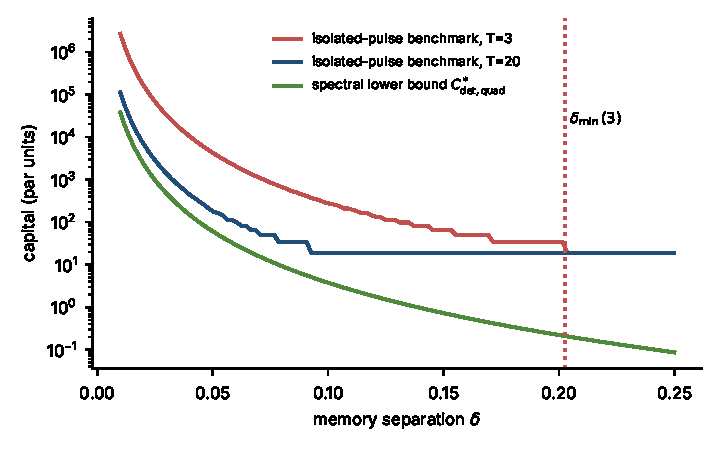
\includegraphics[width=0.62\textwidth]{figs/fig_phase.pdf}
\caption{Capital against separation: isolated-pulse benchmarks with three and twenty observations per pulse, and the spectral lower bound of Theorem~\ref{thm:spectral}. The dotted line is the single-tap resolution floor $\delta_{\min}(3)=0.2028$. Recomputed in this revision.}\label{fig:phase}
\end{figure} These are costs within an isolated-pulse design class, not minimum capital; the next subsection replaces the formula by a ledger.

\subsection{Account-level capital and the gap to the lower bound}

We run each candidate design through an explicit synthetic ledger at reference price $P_*=100$: fills at the average linear-book price, taker fees of 4 basis points, marks at the prevailing price, and 0.5\% maintenance margin. Initial capital is $C_0=\max_t({\rm margin}_t-{\rm equity}_t)$, maximized over both hypotheses, and the test uses the full price path including unwind legs.

\begin{table}[t]\centering\small
\begin{threeparttable}
\caption{Account-level initial capital at $\delta=0.05$ (par units)}\label{tab:ledger}
\setlength{\tabcolsep}{4pt}
\begin{tabular}{lrrrrrr}
\toprule
Design & $C_0$ & Error & End inv. & Peak margin & Max $|v_t|$ & Trades\\
\midrule
12 buys, $T=20$ apart, never unwound & 229.13 & 0.0578 & 75.00 & 39.38 & 6.25 & 12\\
6 buy/sell round trips & 189.45 & 0.0308 & 0.00 & 3.28 & 6.25 & 12\\
5 buy/sell round trips & 157.89 & 0.0442 & 0.00 & 3.28 & 6.25 & 10\\
12 buys, each unwound after 20 steps & 378.82 & 0.0040 & 0.00 & 3.28 & 6.25 & 24\\
Generalized-eigenvector probe ($L=120$) & 65.06 & 0.0500 & 0.00 & 2.74 & 1.24 & 120\\
Generalized-eigenvector probe ($L=160$) & 64.86 & 0.0500 & 0.00 & 2.17 & 1.09 & 160\\
Fee-refined probe ($L=240$) & 64.48 & 0.0500 & 0.00 & --- & 1.30 & 240\\
\bottomrule
\end{tabular}
\begin{tablenotes}\footnotesize\item The pulse designs place a pulse every 40 steps and close it 20 steps later; the fee-refined probe is re-optimized by sequential quadratic programming over $L=240$. The numerically evaluated lower bound of Theorem~\ref{thm:spectral} is 61.41; the explicit constant of Lemma~\ref{thm:capital} is $4.9\times10^{-4}$.\end{tablenotes}
\end{threeparttable}
\end{table}

Table~\ref{tab:ledger} gives three conclusions. First, twelve buys that are never unwound fail the 5\% target once the test uses the joint price path (divergence $4.95<5.41$) and end with 75 units of inventory. Second, if every unwind leg is itself informative, five or six round trips meet the target with zero terminal inventory. Third, pulses are not optimal: a generalized-eigenvector probe, which maximizes divergence per unit of fee-free round-trip cost, needs about 65 par units with maximum trade 1.25 and maximum displacement 2.23, well inside limits.

For flat fee-paying policies $v\in\R^L$ with $\sum_tv_t=0$, the capital problem is
\begin{equation}\label{eq:capprob}
\min_v\ \max_{i\in\{0,1\}}L_i(v)+\sum_t\phi P_*|v_t|+\max_t\mu P_*|I_t|\quad\text{s.t.}\quad\|(H_1-H_0)v\|_2\ge2\sigma z_{1-\alpha},
\end{equation}
where $L_i(v)=\tfrac12v^\top T_{h_i}v$ is the exact Toeplitz round-trip loss. Zero-padding embeds horizon $L$ into $L+1$ at identical cost and information, so the minimum is non-increasing in $L$.

\begin{theorem}[Spectral dissipation lower bound]\label{thm:spectral}
Let $\hat H_i(z)=\sum_{j\ge0}h_{i,j}z^{-j}$, $\Delta\hat H=\hat H_1-\hat H_0$, and define the dissipation kernel
\begin{equation}\label{eq:gdiss}
g_i(\omega)=\mathrm{Re}\,\hat H_i(e^{i\omega})-\kappa/2>0\qquad\forall\omega\in[-\pi,\pi].
\end{equation}
\begin{enumerate}[label=(\roman*)]
\item \emph{Toeplitz energy identity.} For any flat round trip, $L_i(v)=\frac1{2\pi}\int_{-\pi}^{\pi}g_i(\omega)|V(e^{i\omega})|^2d\omega$.
\item \emph{Lower bound.} $\|(H_1-H_0)v\|_2^2\le\sup_\omega\frac{|\Delta\hat H(e^{i\omega})|^2}{g_i(\omega)}L_i(v)$, so every deterministic round trip with error at most $\alpha$ has
\begin{equation}\label{eq:Cdet}
L_i(v)\;\ge\;4\sigma^2z_{1-\alpha}^2\inf_\omega\frac{g_i(\omega)}{|\Delta\hat H(e^{i\omega})|^2}\;\equiv\;C^*_{\rm det,quad}(\delta).
\end{equation}
\item \emph{Bracket.} At $\delta=0.05$, $C^*_{\rm det,quad}=61.14$ at $\omega^*=0.2526$; adding the unavoidable fee $\phi P_*\cdot2\sigma z/\sup_\omega|\Delta\hat H|$ gives the numerical lower estimate $C_{\rm det}\ge61.41$. A feasible 240-step sequence attains 64.48, so the fee-paying optimum lies in $[61.41,64.48]$.
\item \emph{Process noise.} Let the price also receive the innovations $w_t\sim N(0,\sigma_w^2)$ of \eqref{eq:price}, independent of observation noise $\nu_t\sim N(0,\sigma_\nu^2)$, so that from the reset state the observer sees $\tilde x_t=(h_i*v)_t+\kappa^{-1}(h_i*w)_t+\nu_t$, $t<T$. For the known pair of Theorem~\ref{thm:quantity}, put $\sigma_{\rm eff}^2=\sigma_\nu^2+\sigma_w^2/4$, $\bar M=1/(1-S)$ and $C_w=2\sigma_w^4\bar M^2K_*^2(\sigma_\nu^2+\sigma_w^2\bar M^2)/(\kappa^2\sigma_\nu^2\sigma_{\rm eff}^4)$. Every deterministic round trip whose test has errors $\alpha$ and $\beta$ under the two hypotheses satisfies
\begin{equation}\label{eq:Cnoise}
L_i(v)\;\ge\;2\sigma_{\rm eff}^2\bigl[{\rm kl}(\alpha,1-\beta)-C_wT\delta^4\bigr]_+\inf_\omega\frac{g_i(\omega)}{|\Delta\hat H(e^{i\omega})|^2},
\end{equation}
with ${\rm kl}$ as in Theorem~\ref{thm:adaptive}. In-loop noise therefore leaves the $\delta^{-4}$ capital order intact for every horizon $T\le{\rm kl}(\alpha,1-\beta)/(2C_w\delta^4)$; at horizons of order $\delta^{-4}$ and longer, the noise itself separates the pair without a probe (Theorem~\ref{prop:passive}).
\end{enumerate}
\end{theorem}

\begin{figure}[t]\centering
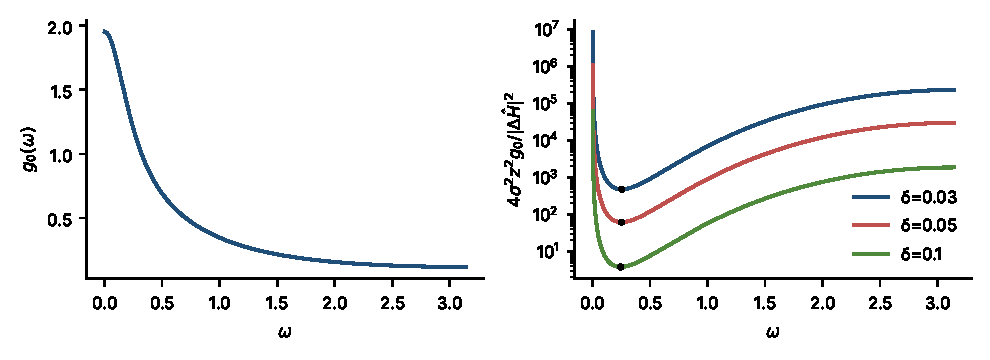
\includegraphics[width=\textwidth]{figs/fig_dissipation.pdf}
\caption{Left: the dissipation kernel $g_0(\omega)$ is strictly positive. Right: the capital ratio in \eqref{eq:Cdet}; dots mark its minimum, near $\omega^*\approx0.25$ for every separation. Recomputed in this revision.}\label{fig:dissip}
\end{figure}

Positivity of $g_i$ follows from Lemma~\ref{lem:cm}: $g_i(\omega)=\tfrac12\sum_\ell\omega_\ell\frac{1-\lambda_\ell^2}{1-2\lambda_\ell\cos\omega+\lambda_\ell^2}>0$. We compute $C^*_{\rm det,quad}$ across separations (Table~\ref{tab:capbounds}): $61.14$ at $\delta=0.05$, with $\delta^4C^*_{\rm det,quad}$ between $3.67\times10^{-4}$ and $3.84\times10^{-4}$, confirming the $\delta^{-4}$ law. The fee term, the feasible upper bounds and the adaptive bound of Theorem~\ref{thm:adaptive} are reported in the same table.

\begin{theorem}[Adaptive and sequential probing]\label{thm:adaptive}
Let $(v_t)_{t\le\tau}$ be any non-anticipating policy adapted to the price filtration, with an almost surely finite stopping time and $\sum_{t\le\tau}v_t=0$. Then
\begin{equation}\label{eq:adaptive}
\E_0[L_0(v)]\;\ge\;2\sigma^2\,{\rm kl}(\alpha,1-\beta)\inf_\omega\frac{g_0(\omega)}{|\Delta\hat H(e^{i\omega})|^2},
\end{equation}
where ${\rm kl}(\alpha,1-\beta)=\alpha\log\tfrac{\alpha}{1-\beta}+(1-\alpha)\log\tfrac{1-\alpha}{\beta}$.
Hence adaptation can lower expected fee-free loss by at most the factor ${\rm kl}(\alpha,1-\beta)/(2z_{1-\alpha}^2)\approx0.4897$ at $\alpha=\beta=0.05$, and cannot alter the $\delta^{-4}$ order.
\end{theorem}

At $\delta=0.05$ the adaptive bound is $29.94$, or $30.22$ with the minimal fee. Pairing it with the feasible deterministic 64.48 gives a numerical ratio of at least $0.464$. In 20{,}000 simulated sequential probability-ratio tests, which split the optimal probe into ten copies of equal information, mean loss was $39.5$ under $H_0$, between the two bounds, but losses vary with the stopping time: the 95th and 99th percentiles of required account capital were $91.7$ and $128.4$, and funding a trader with only the mean loss gives a 37.5\% insolvency rate before the test ends. Expected-loss savings are not solvency savings.

\begin{table}[t]\centering\small
\begin{threeparttable}
\caption{Capital lower bounds and feasible upper bounds across separations (par units)}\label{tab:capbounds}
\begin{tabular}{lcccccc}
\toprule
$\delta$ & $\omega^*$ & $C^*_{\rm det,quad}$ & $\delta^4C^*_{\rm det,quad}$ & Certified $C_{\rm det}$ & Feasible UB & Adaptive LB\\
\midrule
0.02 & 0.2546 & 2397.85 & $3.84\times10^{-4}$ & 2399.58 & 2428.25 & 1176.04\\
0.03 & 0.2541 & 473.19 & $3.83\times10^{-4}$ & 473.97 & 484.50 & 232.51\\
0.05 & 0.2526 & 61.14 & $3.82\times10^{-4}$ & 61.41 & 64.48 & 30.22\\
0.08 & 0.2488 & 9.26 & $3.79\times10^{-4}$ & 9.37 & 10.38 & 4.64\\
0.10 & 0.2453 & 3.77 & $3.77\times10^{-4}$ & 3.83 & 4.44 & 1.91\\
0.15 & 0.2331 & 0.73 & $3.67\times10^{-4}$ & 0.76 & 1.01 & 0.38\\
\bottomrule
\end{tabular}
\begin{tablenotes}\footnotesize\item Calibration $a=0.5$, $\kappa=0.8$, $q=0.2$, $\eta=0.4$, $\sigma=0.01$, $\alpha=0.05$. From \texttt{recompute\_theory.py} and \texttt{recompute\_p1\_capital.py}; the numerical-bound column adds the fee lower bound to the fee-free infimum; the feasible column is the best flat probe found over $L\le240$; the adaptive column adds the fee lower bound to the adaptive bound.\end{tablenotes}
\end{threeparttable}
\end{table}

\begin{theorem}[Finite-horizon Rayleigh--H\"older duality]\label{thm:rh}
For a horizon of $L\ge4$ trading periods, let $E\in\R^{L\times(L-1)}$ be the first-difference basis of flat probes ($\sum_tv_t=0$), $Q_i=\tfrac12T_{h_i}$ (so that $L_i(v)=v^\top Q_iv$), $A_{\rm diff}=(H_1-H_0)^\top(H_1-H_0)$, and let $G_i=E^\top Q_iE\succ0$ and $M=E^\top A_{\rm diff}E\succeq0$ be the reduced execution-loss and information matrices, with $G_i$-orthonormal generalized eigenvectors $e_j$ and eigenvalues $0\le\lambda_1\le\cdots\le\lambda_{L-3}<\lambda_{L-2}\le\lambda_{L-1}$; put $c_{\rm req}=4\sigma^2z_{1-\alpha}^2$ and $c_{\rm fee}=\phi P_*$. For $\theta\in[0,\pi)$ let $d(\theta)=\cos\theta\,e_{L-2}+\sin\theta\,e_{L-1}$, $\lambda(\theta)=\lambda_{L-2}\cos^2\theta+\lambda_{L-1}\sin^2\theta$, $s_\theta={\rm sign}(Ed(\theta))$, and
\begin{equation}\label{eq:rhdefs}
\begin{gathered}
F_{\rm dom}(\theta)=c_{\rm fee}\sqrt{\frac{c_{\rm req}}{\lambda(\theta)}}\,\|Ed(\theta)\|_1,\qquad W_\perp(\theta)=c_{\rm fee}^2\sum_{j\le L-3}\frac{(s_\theta^\top Ee_j)^2}{1-\lambda_j/\lambda(\theta)},\\
\gamma(\theta)=\frac{\lambda(\theta)\,\lambda_{L-3}}{(\lambda(\theta)-\lambda_{L-3})\,c_{\rm req}} .
\end{gathered}
\end{equation}
Then every flat probe meeting the separation constraint of \eqref{eq:capprob} satisfies
\begin{equation}\label{eq:rh}
L_i(v)+c_{\rm fee}\|v\|_1\;\ge\;\min_{\theta}\Bigl\{\frac{c_{\rm req}}{\lambda(\theta)}+\Psi(\theta)\Bigr\}\;\equiv\;C_{\rm RH}(L)\;\ge\;\frac{c_{\rm req}}{\lambda_{L-1}},
\end{equation}
\[
\Psi(\theta)=\min_{x\ge0}\Bigl\{x^2+\Bigl[F_{\rm dom}(\theta)\bigl(1-\gamma(\theta)x^2\bigr)_+-\sqrt{W_\perp(\theta)}\,x\Bigr]_+\Bigr\}\;\ge0 ,
\]
a piecewise-quadratic minimization in closed form; when $\gamma F_{\rm dom}<1$ and the minimizer has $\gamma x^2\le1$, $\Psi=\max\bigl(0,F_{\rm dom}-W_\perp/(4(1-\gamma F_{\rm dom}))\bigr)$.
\end{theorem}

The bound is computable for any horizon. Table~\ref{tab:rh} reports its quadratic part $c_{\rm req}/\lambda_{L-1}$, which decays toward the infinite-horizon value 61.14 at rate $O(L^{-1})$, the full bound $C_{\rm RH}(L)$, and the best feasible fee-paying probe we find at each horizon. At $L=80$ the full bound is $64.72$ against a best probe of $64.76$ on the same loss-plus-fee objective, so the dual is essentially tight at short horizons; at longer horizons the fee term of the dual weakens and the bracket widens to about 5\%. The fee of unpadded full-support eigenvectors grows as $\Theta(\sqrt L)$, which is why zero-padded or $L_1$-localized probes are needed at long horizons.

\begin{table}[t]\centering\small
\begin{threeparttable}
\caption{Finite-horizon capital at $\delta=0.05$ (par units)}\label{tab:rh}
\setlength{\tabcolsep}{4pt}
\begin{tabular}{lcccc}
\toprule
Horizon $L$ & Quadratic part $c_{\rm req}/\lambda_{L-1}$ & Full bound $C_{\rm RH}(L)$ & Best feasible probe & Gap to $C_{\rm det}=61.41$\\
\midrule
80 & 62.55 & 64.72 & 65.02 & 5.9\%\\
120 & 61.84 & 63.39 & 64.59 & 5.2\%\\
160 & 61.54 & 62.46 & 64.50 & 5.0\%\\
240 & 61.32 & 61.76 & 64.48 & 5.0\%\\
320 & 61.25 & --- & $\le64.48$ & $\le5.0\%$\\
480 & 61.19 & --- & $\le64.48$ & $\le5.0\%$\\
\bottomrule
\end{tabular}
\begin{tablenotes}\footnotesize\item Quadratic bound $c_{\rm req}/\lambda_L$ from the generalized eigenproblem of Theorem~\ref{thm:rh} on flat probes (equivalently $c_{\rm req}/(2\lambda'_L)$ with $\lambda'$ computed against $T_{h_0}$ rather than $\tfrac12T_{h_0}$); it converges to the infinite-horizon value 61.14. The full bound minimizes \eqref{eq:rh} over 3{,}600 values of $\theta$ (\texttt{hardening/rh\_bound.py}); at $L=80$ and $120$ a direct numerical minimization of loss plus fee under the separation constraint gives $64.76$ and $64.43$, above the bound. Feasible probes: top generalized eigenvector refined by sequential quadratic programming on the full ledger; at $L=320$ and $480$ the $L=240$ probe padded with zeros is feasible at the same cost, so the best feasible value can only be lower. \end{tablenotes}
\end{threeparttable}
\end{table}

\subsection{Robustness: heteroskedastic impact and probing protocols}

\begin{corollary}[Invariance under impact-induced heteroskedasticity]\label{cor:garch}
Suppose probing inflates innovation variance as $\sigma^2_{i,t}(v)=\sigma^2(1+\xi[(h_i*v)_t]^2)$ and slippage scales as $\kappa_{\rm eff}=\kappa(1+\xi_0|v_t|)$. For capacity-bounded probes, $\KL(P_0^v\|P_1^v)\le\frac{1+O(\xi^2V_{\rm eff}^2)}{2\sigma^2}\|(H_1-H_0)v\|_2^2=O(\|v\|_2^2\delta^4)$, and convex impact only raises dissipation. Required capital remains $\Theta(\delta^{-4})$.
\end{corollary}

Four probing protocols (unconstrained single pulse, repeated capped pulses, a sequential test with dynamic throttling, and a predetermined generalized-eigenvector trajectory) all show capital slopes near $-4$ in $\log\delta$: $-3.90$, $-3.84$, $-3.47$ and $-3.81$ over $\delta\in[0.03,0.12]$, where the sequential slope is flattened by the 1.7 pulses needed at $\delta=0.12$ (Appendix Table~\ref{tab:protocols}). At equal observation horizon, sequential stopping saves 14--49\% of capital relative to repeated capped pulses, but most of the apparent saving from the single-tap baseline comes from observing the transient response, not from adaptivity.

\subsection{From par units to Bitcoin dollars}\label{sec:dollars}

Capital scales as $\sigma^2\delta^{-4}$, so the dollar magnitude hinges on the observation noise. Treating the 4 USDT ten-second price volatility as observation noise would give 9.8 million USDT at $\delta=0.05$, but that conflates price volatility with measurement error. We now estimate observation noise from Binance BTCUSDT one-second closes on January 10--20, 2023, with the Roll covariance estimator $\hat\sigma=\sqrt{-{\rm cov}(\Delta p_t,\Delta p_{t-1})}$ \citep{roll1984}. Daily estimates range from $0.09$ to $0.77$ USDT, median $0.40$ USDT.

\begin{table}[t]\centering
\begin{threeparttable}
\caption{Capital lower bound under alternative observation-noise calibrations (USDT)}\label{tab:capital}
\begin{tabular}{lrrr}
\toprule
Noise calibration & $\delta=0.02$ & $\delta=0.05$ & $\delta=0.10$\\
\midrule
Roll estimator, median (0.40 USDT) & 3{,}874{,}696 & 99{,}193 & 6{,}200\\
One-second price-change s.d., median (1.98 USDT) & 93{,}688{,}369 & 2{,}398{,}422 & 149{,}902\\
Earlier assumption (4 USDT, upper scenario) & 383{,}812{,}500 & 9{,}825{,}600 & 614{,}100\\
\bottomrule
\end{tabular}
\begin{tablenotes}\footnotesize
\item $C(\sigma,\delta)=61.41\times(\sigma/0.01)^2\times(0.05/\delta)^4$, with $\sigma$ the unrounded median. Noise estimated on 11 days of checksum-verified Binance BTCUSDT one-second klines. \end{tablenotes}
\end{threeparttable}
\end{table}

\begin{table}[t]\centering\small
\begin{threeparttable}
\caption{Daily observation-noise estimates, Binance BTCUSDT one-second closes}\label{tab:roll}
\begin{tabular}{lccc}
\toprule
Date & Roll $\hat\sigma$ (USDT) & One-second change s.d.\ (USDT) & Mean price (USDT)\\
\midrule
2023-01-10 & 0.152 & 0.679 & 17{,}288\\
2023-01-11 & 0.092 & 0.891 & 17{,}456\\
2023-01-12 & 0.232 & 2.292 & 18{,}343\\
2023-01-13 & 0.348 & 1.762 & 19{,}075\\
2023-01-14 & 0.773 & 3.511 & 20{,}818\\
2023-01-15 & 0.482 & 1.790 & 20{,}778\\
2023-01-16 & 0.629 & 2.357 & 21{,}036\\
2023-01-17 & 0.457 & 1.976 & 21{,}194\\
2023-01-18 & 0.695 & 2.541 & 21{,}122\\
2023-01-19 & 0.402 & 1.316 & 20{,}850\\
2023-01-20 & 0.316 & 2.038 & 21{,}306\\
\midrule
Median & 0.402 & 1.976 & \\
\bottomrule
\end{tabular}
\begin{tablenotes}\footnotesize\item The Roll estimator measures the negative first-order autocovariance of price changes, which reflects bid-ask bounce and recording noise rather than price volatility.\end{tablenotes}
\end{threeparttable}
\end{table}

\begin{figure}[t]\centering
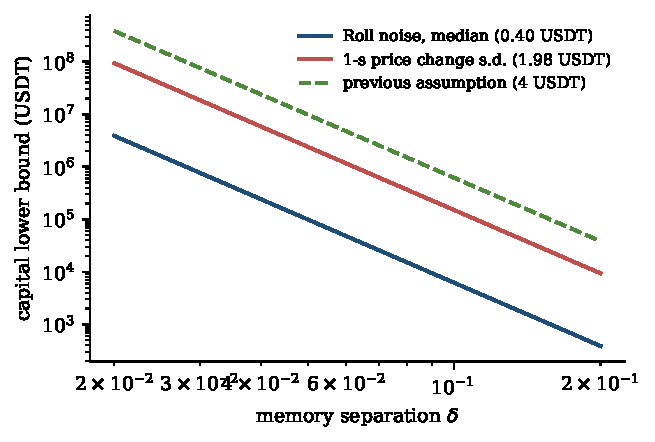
\includegraphics[width=0.62\textwidth]{figs/fig_capital.pdf}
\caption{Capital lower bound against memory separation for three observation-noise calibrations.}\label{fig:capital}
\end{figure}

At realistic noise, separating rates that differ by $0.05$ costs about $9.9\times10^4$ USDT, which is not prohibitive for a well-capitalized desk (Table~\ref{tab:capital}). The barrier becomes large only for finer separation ($3.9$ million USDT at $\delta=0.02$) and, through Theorem~\ref{thm:kcohort}, when several cohorts are unknown. Two factors we do not model would raise these figures: walking several levels of a real book costs more than the linear top-of-book impact assumed here, and impact-induced heteroskedasticity raises the noise a probe must overcome. The capital figures are therefore lower bounds for the stated model.
